\documentclass[conference]{IEEEtran}
\usepackage{amsmath,amsfonts,amssymb}
\usepackage{array}
\usepackage{textcomp}
\usepackage{url}
\usepackage{graphicx}
\usepackage[caption=false,font=footnotesize]{subfig}
\usepackage{booktabs}
\usepackage{algorithm}
\usepackage{algpseudocode}
\usepackage[colorlinks=true, linkcolor=blue, citecolor=blue, urlcolor=blue]{hyperref}
\usepackage{cite}
\usepackage{bm}

\begin{document}
%Broadcast Beam-Steered Optical Wireless Positioning:\\3D Localization Without Cooperative Alignment
%Broadcast 3D Indoor Positioning with a Single Beam-Steered LED and IMU-Assisted Distance Recovery
%Model-Based Beam-Steered Optical Wireless Positioning with Single-LED Single-Photodiode for 3D Localization
\title{Broadcast 3D Indoor Positioning with a Single Beam-Steered LED}
\author{
Kevin Acuna-Condori*, Bastien B\'{e}chadergue*, Hongyu Guan*, and Luc Chassagne*\\
*Laboratoire d'Ing\'{e}nierie des Syst\`{e}mes de Versailles\\
Universit\'{e} Paris-Saclay, UVSQ, 78140 V\'{e}lizy-Villacoublay, France\\
Email: \{kevin-jose.acuna-condori, bastien.bechadergue, hongyu.guan, luc.chassagne\}@uvsq.fr
}
\maketitle

\begin{abstract}
Beam-steered optical wireless positioning with a single LED and a single photodiode can achieve centimeter-level 3D localization, but existing architectures require a cooperative beam-aligned measurement to recover distance, precluding simultaneous multi-user operation.
This paper proposes a broadcast architecture that recovers the 3D position from the same $K$ steered-orientation power measurements used for direction finding, by exploiting the receiver orientation provided by an inertial measurement unit.
We derive the broadcast position error bound (PEB$_\mathrm{B}$)---the Cram\'{e}r--Rao lower bound under $K$ observations with known receiver orientation---and propose a closed-form amplitude estimator that, combined with nonlinear least-squares direction finding, achieves the bound within a factor of $1.01\times$.
Simulations confirm an RMS error of 1.74\,cm with $K{=}9$ orientations and demonstrate simultaneous 3D localization of three heterogeneous receivers from a single LED scan.
\end{abstract}

\begin{IEEEkeywords}
Beam steering, broadcast positioning, Cram\'{e}r--Rao bound, optical wireless positioning, single LED.
\end{IEEEkeywords}

% *******************************************
\section{Introduction}
\label{sec:intro}
% *******************************************

\IEEEPARstart{I}{ndoor} positioning is a core enabler for applications ranging from asset tracking and autonomous navigation to location-based services in environments where global navigation satellite systems are unavailable~\cite{Zafari2019, Italiano2025}.
Among the various technologies, optical wireless positioning (OWP) exploits the spatial confinement and deterministic line-of-sight (LOS) propagation of light to achieve centimeter-level accuracy with cost-effective light-emitting diodes (LEDs)~\cite{Wang2024b, Zhu2025}.

The majority of OWP systems follow a multi-LED paradigm, in which three or more fixed LEDs with known positions serve as anchors for trilateration or triangulation~\cite{Plets2019, electronics8111311}.
This approach, however, requires dense luminaire infrastructures, unique per-lamp identifiers, and simultaneous visibility of at least three sources---conditions that may not hold in corridors, warehouses, or sparse-lighting environments~\cite{Cossu2022, Rekkas2023}.
These limitations have motivated research on single-LED positioning systems, which reduce infrastructure requirements at the cost of reduced measurement diversity.
Reported single-LED solutions compensate for the limited information by placing hardware complexity at the receiver: multiple tilted photodiodes (PDs)~\cite{Qin2020, Li2024}, continuous mechanical PD rotation~\cite{Liu2022, Wang2024, Shi2025}, or aiding sensors such as inertial measurement units (IMUs)~\cite{Ma2024}.

A fundamentally different strategy shifts the spatial diversity from the receiver to the transmitter through beam steering.
Recent advances in MEMS micromirror gimbals~\cite{Liu:25}, liquid-crystal deflectors~\cite{Feng2019}, and optical phased arrays~\cite{mi13070990} enable high-speed redirection of a single LED beam, creating temporal diversity that replaces the spatial redundancy of multiple sources.
Building on this principle, Acuna-Condori~\textit{et~al.}~\cite{AcunaTCOM2025} proposed a model-based beam-steered OWP architecture in which a single LED is steered through $K$ predefined orientations; the resulting $K$ received-signal-strength (RSS) variations at a single PD are sufficient to estimate the transmitter-to-receiver direction.
A dedicated $(K{+}1)$-th measurement, obtained by cooperatively aligning the LED beam toward the receiver and reorienting the PD to face the transmitter, then recovers the distance for full 3D positioning.

While this cooperative architecture achieves sub-degree direction-finding accuracy and centimeter-level 3D error~\cite{AcunaTCOM2025}, the $(K{+}1)$-th measurement introduces two fundamental limitations:
(i)~the PD must be actively reoriented, adding hardware complexity and latency at the receiver; and
(ii)~each receiver requires its own dedicated beam-aligned measurement, precluding simultaneous localization of multiple users from a single LED scan.
These constraints are incompatible with broadcast operation, in which a single periodic scan should serve an arbitrary number of passive receivers---a scenario of practical interest for multi-robot coordination, warehouse automation, and dense IoT deployments.

In this paper, we propose a broadcast beam-steered OWP architecture that achieves 3D positioning using only the $K$ steered-orientation measurements, without any cooperative alignment or PD reorientation.
The key insight is that the $K$ absolute power levels, which the ratio-based direction estimators deliberately discard, carry distance information through a common amplitude parameter that couples the unknown distance with the receiver incidence angle.
By exploiting the receiver orientation provided by a commercial inertial measurement unit (IMU), this ambiguity is resolved and the distance is recovered in closed form from the same measurements used for direction finding.

The main contributions are:
\begin{enumerate}
    \item A broadcast single-LED OWP architecture that achieves 3D localization from $K$ measurements alone, enabling simultaneous multi-user positioning without per-receiver dedicated measurements.
    \item The broadcast position error bound ($\mathrm{PEB}_\mathrm{B}$): the Cram\'{e}r--Rao lower bound for 3D position estimation from $K$ steered-orientation observations with known receiver orientation, together with a characterization of its dependence on the number of orientations, receiver tilt, and SNR.
    \item A closed-form amplitude estimator derived from the profiled Gaussian likelihood, which, combined with existing NLS direction finding, yields an asymptotically efficient positioning pipeline achieving the $\mathrm{PEB}_\mathrm{B}$.
\end{enumerate}

The remainder of this paper is organized as follows.
Section~\ref{sec:system} presents the system model and the broadcast positioning architecture.
Section~\ref{sec:peb} derives the broadcast position error bound.
Section~\ref{sec:parametric} evaluates the bound as a function of key system parameters.
Section~\ref{sec:estimators} validates the estimator performance through Monte Carlo simulation and multi-user trajectory estimation.
Section~\ref{sec:conclusion} concludes the paper.

% *******************************************
\section{System Model and Broadcast Architecture}
\label{sec:system}
% *******************************************

\subsection{Channel Model}
\label{subsec:channel}

We consider a single beam-steered LED transmitter mounted at a known ceiling position $\mathbf{t}=[0,0,H]^{\mathsf T}$ that sequentially steers its optical axis along $K$ predefined unit-norm orientations $\{\mathbf{n}_{t,i}\}_{i=1}^K$, $\mathbf{n}_{t,i}\in\mathbb{S}^2$.
A single photodiode (PD) receiver is located at an unknown position $\mathbf{r}=[x,y,z]^{\mathsf T}$ with a known orientation $\mathbf{n}_r\in\mathbb{S}^2$ provided by an IMU.
Let $\mathbf{d}=\mathbf{r}-\mathbf{t}$ denote the displacement vector, $d=\lVert\mathbf{d}\rVert$ the transmitter--receiver distance, and $\mathbf{n}_d=\mathbf{d}/d$ the unit direction vector.

For the $i$-th LED orientation, the noise-free received optical power under a Lambertian channel model~\cite{Kahn1997} is:
\begin{equation}
\mu_i(\mathbf{r}) = \frac{(m+1)A_{\mathrm{det}}}{2\pi}\,\frac{P_t}{d^2}\,\cos^m(\phi_i)\,\cos(\psi), \quad \psi\leq\Psi_{\mathrm{FOV}},
\label{eq:mu_full}
\end{equation}
where $m=-\ln 2/\ln(\cos\Phi_{1/2})$ is the Lambertian order, $A_{\mathrm{det}}$ is the PD effective area, $P_t$ is the transmitted optical power, $\Psi_{\mathrm{FOV}}$ is the receiver field of view, and the irradiance and incidence angles are defined by:
\begin{equation}
\cos\phi_i = \frac{\mathbf{n}_{t,i}\cdot\mathbf{d}}{d} \triangleq Q_i, \quad
\cos\psi = \frac{\mathbf{n}_r\cdot(-\mathbf{d})}{d}.
\label{eq:angles}
\end{equation}

Defining the radiometric constant $C\triangleq P_t(m+1)A_{\mathrm{det}}/(2\pi)$ and the amplitude parameter:
\begin{equation}
\eta \triangleq \frac{C\cos\psi}{d^2},
\label{eq:eta_def}
\end{equation}
the observation model compactly factorizes as:
\begin{equation}
\mu_i = \eta\,Q_i^{\,m}, \quad i=1,\ldots,K.
\label{eq:mu_compact}
\end{equation}
The scalar $\eta>0$ is common to all $K$ measurements (since the receiver remains stationary during the $K$-orientation scan) and encapsulates the unknown distance $d$ and the receiver-dependent term $\cos\psi$.

At each orientation~$i$, $N$ independent power samples are acquired. The sample mean $\hat\mu_i = (1/N)\sum_{k=1}^N P_{r,i,k}$ is the minimum-variance unbiased estimator of $\mu_i$ and satisfies:
\begin{equation}
\hat\mu_i \sim \mathcal{N}\bigl(\mu_i,\;\sigma^2/N\bigr),
\label{eq:obs_model}
\end{equation}
where $\sigma^2$ is the per-sample noise variance in the optical power domain.

\subsection{Broadcast Positioning Architecture}
\label{subsec:broadcast_arch}

In~\cite{AcunaTCOM2025}, a cooperative $(K{+}1)$-th measurement---obtained by steering the LED toward $\hat{\mathbf{n}}_d$ and reorienting the PD to $-\hat{\mathbf{n}}_d$---is required to recover the distance~$d$.
This cooperative step precludes simultaneous localization of multiple receivers, since each user requires a dedicated beam-aligned measurement.
The architecture proposed herein eliminates this requirement by recovering~$d$ directly from the same $K$ power observations used for direction finding, provided that $\mathbf{n}_r$ is known.

\subsubsection{Direction Finding}
The transmitter-to-receiver direction $\mathbf{n}_d$ is estimated from $\{\hat\mu_i\}_{i=1}^K$ using the ratio-based estimators developed in~\cite{AcunaTCOM2025}.
The power ratios $\beta_i=(\hat\mu_i/\hat\mu_1)^{1/m}$ cancel the common factor~$\eta$, yielding linear constraints on $\mathbf{n}_d$ that are solved via generalized least squares (GLS) or nonlinear least squares (NLS).
Since $\eta$ is eliminated by the ratio operation, the resulting direction estimate $\hat{\mathbf{n}}_d$ is independent of $\mathbf{n}_r$, $d$, and $P_t$~\cite{AcunaTCOM2025}.

\subsubsection{Broadcast Distance Recovery}
\label{subsubsec:distance_recovery}
Once $\hat{\mathbf{n}}_d$ is available, the absolute power levels are exploited to recover the amplitude parameter~$\eta$ and, subsequently, the distance~$d$.

Under the model~\eqref{eq:mu_compact} with i.i.d.\ Gaussian noise~\eqref{eq:obs_model}, the log-likelihood of $\eta$ for a given direction $\hat{\mathbf{n}}_d$ is:
\begin{equation}
\ell(\eta) = -\frac{N}{2\sigma^2}\sum_{i=1}^K \bigl(\hat\mu_i - \eta\,\hat Q_i^{\,m}\bigr)^2 + \mathrm{const.},
\label{eq:loglik_eta}
\end{equation}
where $\hat Q_i\triangleq\mathbf{n}_{t,i}\cdot\hat{\mathbf{n}}_d$ denotes the direction cosine evaluated at the estimated direction.
The MLE of $\eta$ is obtained by setting $\partial\ell/\partial\eta=0$:
\begin{equation}
\frac{\partial\ell}{\partial\eta} = \frac{N}{\sigma^2}\sum_{i=1}^K \bigl(\hat\mu_i - \eta\,\hat Q_i^{\,m}\bigr)\hat Q_i^{\,m} = 0,
\label{eq:dloglik}
\end{equation}
which, upon expanding and solving for $\eta$, yields the closed-form estimator:
\begin{equation}
\hat\eta = \sum_{i=1}^K \hat\mu_i\,\hat Q_i^{\,m}\;\Big/\;\sum_{i=1}^K \hat Q_i^{\,2m}.
\label{eq:eta_hat}
\end{equation}
This expression admits a geometric interpretation: $\hat\eta$ is the inner product between the observed power vector $[\hat\mu_1,\ldots,\hat\mu_K]^{\mathsf T}$ and the predicted shape vector $[\hat Q_1^m,\ldots,\hat Q_K^m]^{\mathsf T}$, normalized by the squared norm of the latter.
It corresponds to the orthogonal projection of the observation onto the one-dimensional subspace spanned by the Lambertian power profile, and is therefore the minimum-variance unbiased estimator of~$\eta$ conditioned on~$\hat{\mathbf{n}}_d$.

The incidence cosine is computed from the known receiver orientation and the estimated direction:
\begin{equation}
\hat\cos\psi = -\mathbf{n}_r\cdot\hat{\mathbf{n}}_d.
\label{eq:cos_psi_hat}
\end{equation}
Substituting~\eqref{eq:eta_hat} and~\eqref{eq:cos_psi_hat} into the definition~\eqref{eq:eta_def} and solving for $d$ yields the broadcast distance estimate:
\begin{equation}
\hat d = \sqrt{\frac{C\hat\cos\psi}{\hat\eta}}\,,
\label{eq:d_hat}
\end{equation}
and the complete 3D position estimate is:
\begin{equation}
\hat{\mathbf{r}} = \mathbf{t} + \hat d\,\hat{\mathbf{n}}_d.
\label{eq:r_hat}
\end{equation}

\subsubsection{Multi-User Broadcast Operation}
The $K$-orientation LED scan is performed periodically and independently of the number of receivers.
Each receiver~$j$ ($j=1,\ldots,N_{\mathrm{rx}}$) independently collects the $K$ power measurements, applies the direction-finding and distance-recovery pipeline described above using its own $\mathbf{n}_{r,j}$ (from its local IMU), and obtains $\hat{\mathbf{r}}_j$ without any dedicated measurement or feedback to the transmitter.
This constitutes a fully broadcast positioning architecture: one LED scan serves all receivers simultaneously.

% *******************************************
\section{Broadcast Position Error Bound}
\label{sec:peb}
% *******************************************

This section derives the Cram\'{e}r--Rao lower bound (CRLB) for 3D position estimation under the broadcast architecture, termed the broadcast position error bound ($\mathrm{PEB}_\mathrm{B}$).
Unlike bounds that incorporate a dedicated ranging measurement, the $\mathrm{PEB}_\mathrm{B}$ quantifies the fundamental accuracy achievable from the $K$ steered-orientation observations alone when $\mathbf{n}_r$ is known.

\subsection{Fisher Information Matrix}
\label{subsec:fim}

The parameter of interest is the receiver position $\mathbf{r}=[x,y,z]^{\mathsf T}\in\mathbb{R}^3$.
Under the observation model~\eqref{eq:obs_model}, the $K$ sample means $\{\hat\mu_i\}_{i=1}^K$ are independent Gaussian random variables with means $\{\mu_i(\mathbf{r})\}$ given by~\eqref{eq:mu_full} and common variance $\sigma^2/N$.
Applying the Slepian--Bangs formula~\cite{Kay1993}, the $3\times 3$ Fisher information matrix (FIM) for position estimation is:
\begin{equation}
\mathcal{I}_{\mathrm{B}}(\mathbf{r})
= \frac{N}{\sigma^2}\sum_{i=1}^K
  \bigl[\nabla_{\mathbf{r}}\mu_i(\mathbf{r})\bigr]
  \bigl[\nabla_{\mathbf{r}}\mu_i(\mathbf{r})\bigr]^{\!\mathsf T},
\label{eq:fim_broadcast}
\end{equation}
where $\nabla_{\mathbf{r}}\mu_i$ denotes the gradient of the noise-free power with respect to the receiver position.

From~\eqref{eq:mu_full} and~\eqref{eq:angles}, the gradient of the $i$-th observation is~\cite{AcunaTCOM2025}:
\begin{multline}
\nabla_{\mathbf{r}}\mu_i = \frac{C}{d^3}\Bigl[
  m\cos^{m-1}\!(\phi_i)\cos(\psi)\,\mathbf{n}_{t,i} \\
  - \cos^m\!(\phi_i)\,\mathbf{n}_r
  - (m{+}3)\cos^m\!(\phi_i)\cos(\psi)\,\mathbf{n}_d
\Bigr].
\label{eq:grad_mu}
\end{multline}
Each gradient vector~\eqref{eq:grad_mu} has components along three directions: the LED orientation~$\mathbf{n}_{t,i}$ (which provides angular discrimination between orientations), the receiver normal~$\mathbf{n}_r$ (which couples the incidence geometry to the position), and the radial direction~$\mathbf{n}_d$ (which carries distance information through the $1/d^2$ attenuation).
The accumulation of $K$ rank-one outer products in~\eqref{eq:fim_broadcast} yields a full-rank FIM for $K\geq 3$ non-coplanar orientations, establishing that three-dimensional position is identifiable from $K$ broadcast measurements alone.

\subsection{Position Error Bound}
\label{subsec:peb_def}

The broadcast PEB is defined as the square root of the trace of the inverse FIM:
\begin{equation}
\mathrm{PEB}_\mathrm{B}(\mathbf{r})
= \sqrt{\operatorname{tr}\!\bigl\{\mathcal{I}_{\mathrm{B}}^{-1}(\mathbf{r})\bigr\}}.
\label{eq:peb_b}
\end{equation}
This quantity represents the minimum achievable root-mean-square (RMS) position error for any unbiased estimator of $\mathbf{r}$ that uses only the $K$ steered-orientation power measurements with known $\mathbf{n}_r$.
It depends on the receiver position~$\mathbf{r}$ (through $d$, $\cos\psi$, and $\{Q_i\}$), the orientation set $\{\mathbf{n}_{t,i}\}$, the receiver orientation $\mathbf{n}_r$, and the system parameters $(N, \sigma^2, m, P_t, A_{\mathrm{det}})$.

\subsection{Dependence on Receiver Orientation}
\label{subsec:peb_nr_dep}

A distinguishing property of the broadcast bound is its dependence on the receiver orientation~$\mathbf{n}_r$.
This dependence enters through two mechanisms in the gradient~\eqref{eq:grad_mu}: (i)~the explicit term $-\cos^m(\phi_i)\,\mathbf{n}_r$, and (ii)~the implicit dependence of $\cos\psi = -\mathbf{n}_r\cdot\mathbf{n}_d$ which scales the remaining terms.

Physically, a tilted receiver collects less optical power ($\cos\psi < 1$), reducing the signal-to-noise ratio and diminishing the magnitude of the gradient vectors.
As a consequence, the FIM~\eqref{eq:fim_broadcast} contracts and the $\mathrm{PEB}_\mathrm{B}$ increases.
This contrasts with the direction-finding stage, which is provably $\mathbf{n}_r$-independent~\cite{AcunaTCOM2025} due to the cancellation of~$\eta$ in the ratio formulation.
The broadcast distance-recovery stage, by contrast, relies on the absolute power level $\eta = C\cos\psi/d^2$, which explicitly involves $\mathbf{n}_r$.

The sensitivity of $\mathrm{PEB}_\mathrm{B}$ to receiver tilt is quantified in Section~\ref{sec:parametric} and constitutes a key design parameter: it establishes the IMU accuracy requirement for broadcast positioning.

\subsection{Identifiability and Rank Conditions}
\label{subsec:identifiability}

The FIM $\mathcal{I}_{\mathrm{B}}(\mathbf{r})$ is the sum of $K$ rank-one matrices.
A necessary condition for $\mathcal{I}_{\mathrm{B}}$ to be full rank (and hence for $\mathrm{PEB}_\mathrm{B}$ to be finite) is that the gradient vectors $\{\nabla_{\mathbf{r}}\mu_i\}_{i=1}^K$ span $\mathbb{R}^3$.
From~\eqref{eq:grad_mu}, each gradient lies in the subspace spanned by $\{\mathbf{n}_{t,i}, \mathbf{n}_r, \mathbf{n}_d\}$.
With $K\geq 3$ orientations that are not coplanar with $\mathbf{n}_d$, the gradients span the full three-dimensional space and the position is uniquely identifiable.
For $K\leq 2$, the FIM is rank-deficient and $\mathrm{PEB}_\mathrm{B}\to\infty$.
In the overdetermined regime ($K\geq 4$), redundant observations improve the conditioning of~$\mathcal{I}_{\mathrm{B}}$ and monotonically reduce the bound.

% *******************************************
\section{Parametric Analysis}
\label{sec:parametric}
% *******************************************

This section evaluates the $\mathrm{PEB}_\mathrm{B}$ as a function of three key system parameters: the number of orientations~$K$, the receiver tilt angle~$\theta_{\mathrm{tilt}}$, and the signal-to-noise ratio (SNR).
The analysis is conducted over a $3\times3\times2$\,m$^3$ room with the LED at the ceiling center ($\mathbf{t}=[0,0,2]^{\mathsf T}$\,m).
The receiver testbed comprises $|\mathcal{R}|=1{,}792$ uniformly spaced positions at $x,y\in[-1.5,1.5]$\,m and $z\in[0,1.2]$\,m (step~$0.2$\,m).
Unless stated otherwise, the system parameters are: $P_t=0.405$\,W, $\Phi_{1/2}=45^\circ$, $A_{\mathrm{det}}=26.4$\,mm$^2$, $\Psi_{\mathrm{FOV}}=85^\circ$, $N=1{,}000$ samples per orientation, $\sigma^2=3\times10^{-14}$\,W$^2$, and $\mathbf{n}_r=[0,0,1]^{\mathsf T}$.
The orientation sets $\{\mathbf{n}_{t,i}\}_{i=1}^K$ are those optimized for the direction error bound (DEB) in~\cite{AcunaTCOM2025}.

\subsection{Spatial Distribution of the Broadcast PEB}
\label{subsec:heatmap}

Figure~\ref{fig:heatmap} shows the spatial distribution of $\mathrm{PEB}_\mathrm{B}$ across the $3\times3$\,m$^2$ floor at a receiver height of $z=0.8$\,m for $K=5$ and $K=9$ orientations.
The bound is lowest near the room center, directly below the LED, where the incidence angle $\psi$ is small and the irradiance cosines $\{Q_i\}$ are large, yielding high SNR and well-conditioned gradients.
Toward the room boundaries and corners, the bound increases due to the combined effect of larger incidence angles (reducing $\cos\psi$) and reduced angular discrimination as the receiver approaches the edge of the LED's field of view.
Increasing $K$ from~5 to~9 produces a uniform reduction in $\mathrm{PEB}_\mathrm{B}$ across the entire floor, with the improvement most pronounced at the boundaries where the additional orientations provide supplementary gradient diversity.

\begin{figure}[t]
    \centering
    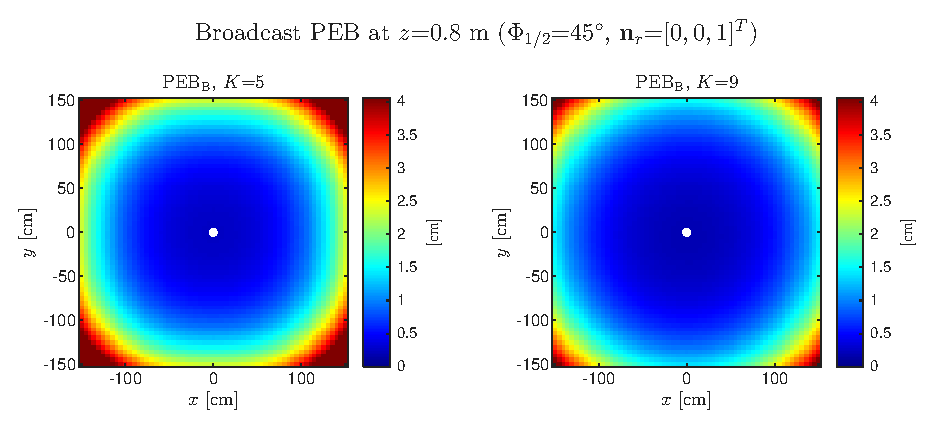
\includegraphics[width=\linewidth]{../simulations/results/Fig01_PEB_B_heatmap}
    \caption{Spatial distribution of $\mathrm{PEB}_\mathrm{B}$ at $z=0.8$\,m for $K=5$ (left) and $K=9$ (right). The LED is at the ceiling center (white dot). The colour scale is shared and clipped at 4\,cm.}
    \label{fig:heatmap}
\end{figure}

\subsection{Effect of the Number of Orientations}
\label{subsec:effect_K}

Figure~\ref{fig:peb_vs_K} reports the RMS of $\mathrm{PEB}_\mathrm{B}$ over all testbed positions as a function of~$K$ for $K\in\{3,\ldots,15\}$.
The bound decreases monotonically with~$K$, reflecting the additional Fisher information contributed by each orientation through a new rank-one term in the FIM~\eqref{eq:fim_broadcast}.
The improvement is steepest for small~$K$: increasing from $K=3$ to $K=5$ reduces the RMS-$\mathrm{PEB}_\mathrm{B}$ from approximately 8.1\,cm to 2.5\,cm, whereas the gain from $K=9$ to $K=15$ is less than 0.4\,cm.
This diminishing-return behaviour is consistent with the FIM structure: each additional orientation contributes a gradient vector that becomes increasingly collinear with the subspace already spanned by the existing $K$ gradients.
For the operating point $K=9$, the RMS-$\mathrm{PEB}_\mathrm{B}$ reaches 1.7\,cm, indicating that centimeter-level 3D accuracy is achievable in the broadcast regime.

\begin{figure}[t]
    \centering
    
\includegraphics[width=0.9\linewidth]{../simulations/results/Fig02_PEB_vs_K}
    \caption{RMS-$\mathrm{PEB}_\mathrm{B}$ versus $K$ over the 3D testbed ($\Phi_{1/2}=45^\circ$, $\mathbf{n}_r=[0,0,1]^{\mathsf T}$).}
    \label{fig:peb_vs_K}
\end{figure}

\subsection{Sensitivity to Receiver Tilt}
\label{subsec:effect_tilt}

The dependence of $\mathrm{PEB}_\mathrm{B}$ on the receiver orientation, established analytically in Section~\ref{subsec:peb_nr_dep}, is quantified in Fig.~\ref{fig:peb_vs_tilt}.
The receiver is tilted by an angle $\theta_{\mathrm{tilt}}$ from the vertical, with the tilt azimuth uniformly averaged over $[0^\circ, 360^\circ)$ to represent an arbitrary tilt direction.
For each~$\theta_{\mathrm{tilt}}$, the RMS-$\mathrm{PEB}_\mathrm{B}$ is computed by first averaging the squared bound over azimuth at each position (yielding the effective per-position bound) and then computing the spatial RMS over the testbed.

For moderate tilt angles ($\theta_{\mathrm{tilt}}\leq 6^\circ$), the degradation remains below 5\% for all~$K$, confirming that the broadcast architecture is compatible with the orientation accuracy provided by commercial inertial measurement units.
Beyond $\theta_{\mathrm{tilt}}=15^\circ$, the degradation accelerates, reaching a factor of ${\approx}3\times$ at $\theta_{\mathrm{tilt}}=30^\circ$ for $K=5$.
This acceleration is driven by two mechanisms: (i)~the reduced incidence cosine ($\cos\psi<1$) diminishes the received power and thus the SNR at every position, and (ii)~at large tilt angles, peripheral receiver positions fall outside the effective field of view ($\psi>\Psi_{\mathrm{FOV}}$), causing a loss of signal and a sharp increase in the local bound.
Increasing~$K$ mitigates the degradation: at $\theta_{\mathrm{tilt}}=30^\circ$, $K=9$ limits the RMS-$\mathrm{PEB}_\mathrm{B}$ to approximately 5.2\,cm compared to 8.0\,cm for $K=5$, as the additional orientations provide redundant measurements that compensate for the reduced SNR.

\begin{figure}[t]
    \centering
    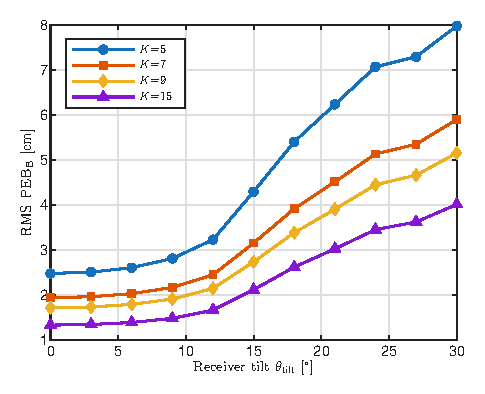
\includegraphics[width=0.9\linewidth]{../simulations/results/Fig_A4_PEB_vs_tilt_rms}
    \caption{RMS-$\mathrm{PEB}_\mathrm{B}$ versus receiver tilt $\theta_{\mathrm{tilt}}$ for $K\in\{5,7,9\}$ ($\Phi_{1/2}=45^\circ$). The tilt azimuth is uniformly averaged. Degradation remains below 5\% for $\theta_{\mathrm{tilt}}\leq 6^\circ$.}
    \label{fig:peb_vs_tilt}
\end{figure}

\subsection{Effect of Signal-to-Noise Ratio}
\label{subsec:effect_snr}

Figure~\ref{fig:peb_vs_snr} presents the RMS-$\mathrm{PEB}_\mathrm{B}$ as a function of the average SNR for $K=9$ (bold curve) and for $K\in\{5,\ldots,15\}$ (shaded band).
On the log--log axes, all curves exhibit a slope of $-1/2$, confirming the theoretical $1/\sqrt{\mathrm{SNR}}$ scaling predicted by the CRLB under Gaussian noise~\cite{Kay1993}.
At the nominal operating point ($\mathrm{SNR}\approx14$\,dB, corresponding to the system parameters listed above), the $K=9$ bound is 1.7\,cm.
The sub-centimeter regime ($\mathrm{PEB}_\mathrm{B}<1$\,cm) is reached at $\mathrm{SNR}\geq 22$\,dB for $K=9$, which is readily achievable in practice for DC power measurements with narrowband filtering or operation in controlled ambient conditions.
The width of the shaded band quantifies the gain from additional orientations at any given SNR; this band narrows at high SNR, indicating diminishing returns from increasing~$K$ in low-noise regimes.

\begin{figure}[t]
    \centering
    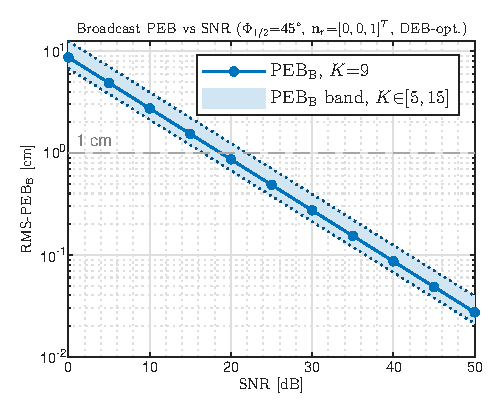
\includegraphics[width=0.9\linewidth]{../simulations/results/Fig_3_PEB_vs_SNR_rms}
    \caption{RMS-$\mathrm{PEB}_\mathrm{B}$ versus SNR ($\Phi_{1/2}=45^\circ$, $\mathbf{n}_r=[0,0,1]^{\mathsf T}$). Bold: $K=9$; shaded band: $K\in[5,15]$; dotted: $K=5$ (upper) and $K=15$ (lower). The dashed line marks 1\,cm.}
    \label{fig:peb_vs_snr}
\end{figure}

% *******************************************
\section{Estimator Performance}
\label{sec:estimators}
% *******************************************

This section validates the broadcast positioning pipeline through Monte Carlo simulation and demonstrates its application to multi-user trajectory estimation.
The simulation parameters are identical to those of Section~\ref{sec:parametric}, with $M=1{,}000$ independent noise realizations per testbed position and the receiver orientation fixed at $\mathbf{n}_r=[0,0,1]^{\mathsf T}$.
Three direction-finding estimators are evaluated---GLS, WLS, and NLS~\cite{AcunaTCOM2025}---each followed by the broadcast distance recovery of Section~\ref{subsubsec:distance_recovery}.

\subsection{Positioning Accuracy}
\label{subsec:accuracy}

Table~\ref{tab:results} reports the 3D positioning metrics for $K\in\{5,9\}$.
The NLS estimator achieves a root-mean-square error (RMSE) of 2.48\,cm at $K=5$ and 1.74\,cm at $K=9$, closely tracking the broadcast bound ($\mathrm{PEB}_\mathrm{B}$: 2.49\,cm and 1.72\,cm, respectively).
This near-unity ratio ($\mathrm{RMSE}_{\mathrm{NLS}}/\mathrm{PEB}_\mathrm{B}\approx 1.00$) confirms that the two-stage pipeline---NLS direction finding followed by amplitude-based distance recovery~\eqref{eq:eta_hat}--\eqref{eq:d_hat}---is asymptotically efficient.
This efficiency arises because NLS jointly estimates the direction and the normalized amplitude through the profiled likelihood, preserving the full Fisher information available in the $K$ observations.

The GLS estimator, which operates on power ratios and thereby discards absolute amplitude information, exhibits a larger gap: RMSE of 3.98\,cm ($K=5$) and 2.46\,cm ($K=9$), corresponding to factors of 1.60$\times$ and 1.43$\times$ above the bound, respectively.
WLS, a diagonal approximation of GLS, further degrades to 4.87\,cm ($K=5$) and 3.60\,cm ($K=9$).
The reversal of the GLS--WLS hierarchy at $K=9$ (WLS becoming worse than GLS, unlike at small~$K$) is consistent with the diagonal covariance approximation becoming increasingly suboptimal as the number of off-diagonal cross-correlation terms grows with~$K$.

\begin{table}[t]
\centering
\caption{Broadcast 3D positioning performance ($M{=}1{,}000$ MC trials, $|\mathcal{R}|{=}1{,}792$ positions, $\mathbf{n}_r{=}[0,0,1]^{\mathsf T}$).}
\label{tab:results}
\begin{tabular}{clccc}
\toprule
$K$ & Method & RMSE [cm] & CDF$_{90\%}$ [cm] & APE [cm] \\
\midrule
5 & GLS   & 3.98 & 5.37 & 2.69 \\
5 & WLS   & 4.87 & 5.35 & 2.83 \\
5 & NLS   & 2.48 & 3.79 & 1.99 \\
5 & $\mathrm{PEB}_\mathrm{B}$ & 2.49 & 3.76 & 2.02 \\
\midrule
9 & GLS   & 2.46 & 3.52 & 1.78 \\
9 & WLS   & 3.60 & 4.72 & 2.36 \\
9 & NLS   & 1.74 & 2.68 & 1.41 \\
9 & $\mathrm{PEB}_\mathrm{B}$ & 1.72 & 2.69 & 1.42 \\
\bottomrule
\end{tabular}
\end{table}

Figure~\ref{fig:cdf} presents the empirical cumulative distribution function (CDF) of the per-position RMSE for all estimators at $K=5$ (solid lines) and $K=9$ (dashed lines).
For $K=9$, the NLS curve is virtually indistinguishable from the $\mathrm{PEB}_\mathrm{B}$ across the entire distribution, confirming that the estimator achieves the bound not only in an average sense but at every spatial position.
All $K=9$ curves stochastically dominate their $K=5$ counterparts, in agreement with the monotonic improvement predicted by the bound analysis of Section~\ref{subsec:effect_K}.

\begin{figure}[t]
    \centering
    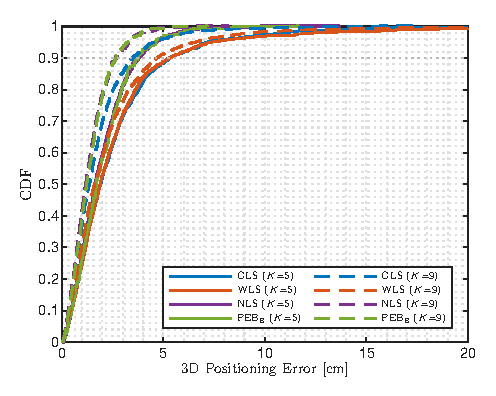
\includegraphics[width=0.9\linewidth]{../simulations/results/broadcast_MC10/Fig05_CDF_broadcast}
    \caption{Empirical CDF of the 3D positioning error for $K=5$ (solid) and $K=9$ (dashed). NLS tracks the $\mathrm{PEB}_\mathrm{B}$ at both operating points; GLS and WLS exhibit structural gaps.}
    \label{fig:cdf}
\end{figure}

\subsection{Multi-User Trajectory Estimation}
\label{subsec:trajectories}

To illustrate the broadcast capability, Fig.~\ref{fig:trajectories} depicts the simultaneous 3D position estimation of three receivers traversing distinct trajectories within the room, using a single $K=9$ LED scan per time instant.
The three use cases represent heterogeneous indoor localization scenarios at different heights:
\begin{itemize}
    \item A robotic vacuum cleaner ($z\approx 0.10$\,m) following a boustrophedon coverage pattern;
    \item A pedestrian carrying a smartphone ($z\approx 0.80$\,m) along a random walking trajectory with natural gait sway;
    \item An automated guided vehicle (AGV) in a warehouse setting ($z\approx 0.50$\,m) following an aisle-based path with 90$^\circ$ turns.
\end{itemize}
Each receiver independently applies the NLS direction-finding and broadcast distance-recovery pipeline using its local IMU-reported orientation.
The estimated positions (star markers) closely overlap the ground-truth trajectories (circle/diamond/triangle markers) across all three heights and trajectory types, with mean positioning errors of approximately 1\,cm for all users.
This result demonstrates that the proposed architecture simultaneously serves receivers at vastly different heights and with fundamentally different mobility patterns, without any dedicated per-user measurement or feedback channel---a capability that is precluded by cooperative beam-aligned architectures.

\begin{figure}[t]
    \centering
    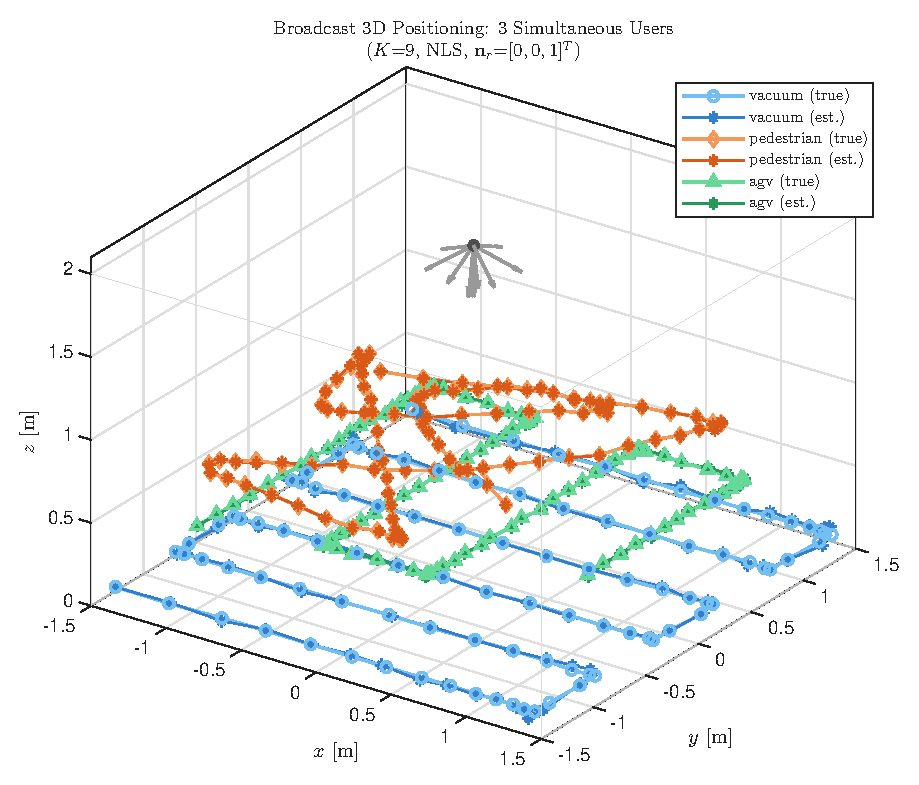
\includegraphics[width=\linewidth]{../simulations/results/Fig_flagship_broadcast_3D}
    \caption{Simultaneous 3D trajectory estimation of three receivers ($K=9$, NLS). Ground truth: open markers; estimates: star markers. The LED and its $K=9$ orientations are shown at the ceiling.}
    \label{fig:trajectories}
\end{figure}

% *******************************************
\section{Conclusion}
\label{sec:conclusion}
% *******************************************

This paper introduced a broadcast beam-steered OWP architecture that achieves 3D indoor localization using only the $K$ steered-orientation power measurements, without the cooperative beam-aligned measurement required by prior work.
The key enabler is the recovery of the transmitter--receiver distance from the absolute power levels via a closed-form amplitude estimator derived from the profiled Gaussian likelihood, combined with the receiver orientation provided by an IMU.

The broadcast position error bound ($\mathrm{PEB}_\mathrm{B}$) was derived as the CRLB for 3D position estimation from $K$ measurements with known receiver orientation.
The parametric analysis established that: (i)~the bound decreases monotonically with~$K$, reaching 1.72\,cm at $K=9$; (ii)~for receiver tilt angles below $6^\circ$ (readily achievable with commercial IMUs), the degradation remains below 5\%; and (iii)~the bound follows the theoretical $1/\sqrt{\mathrm{SNR}}$ scaling, with sub-centimeter accuracy achievable at SNR~$\geq 22$\,dB.

Monte Carlo simulations over 1,792 testbed positions confirmed that the NLS direction estimator, combined with the proposed broadcast distance recovery, achieves the $\mathrm{PEB}_\mathrm{B}$ within a factor of $1.01\times$---demonstrating that the two-stage pipeline is asymptotically efficient without requiring a joint single-stage optimization.
A multi-user demonstration showed that three receivers at different heights (0.1, 0.5, and 0.8\,m)---representing a robotic vacuum, a warehouse AGV, and a pedestrian with a smartphone---are simultaneously localized with centimeter-level accuracy from a single $K$-orientation LED scan, without any per-user dedicated measurement or feedback.

Future work includes experimental validation with mechanical beam steering, joint optimization of the orientation set for the broadcast bound (as opposed to the direction-finding bound used herein), and extension to multi-LED configurations for enhanced coverage and redundancy.

\bibliographystyle{IEEEtran}
\bibliography{References}

\end{document}
